\chapter{Software Architecture}
\label{chapter:architecture}

This chapter will discuss the software design behind this work.  It will cover the underlying tools, and then present the framework broken up into functional modules, rather than presenting the entire framework altogether.

\section{ROS}

I used ROS.  Look it up.

\section{Video input}

\begin{figure}[H]
  \centering
    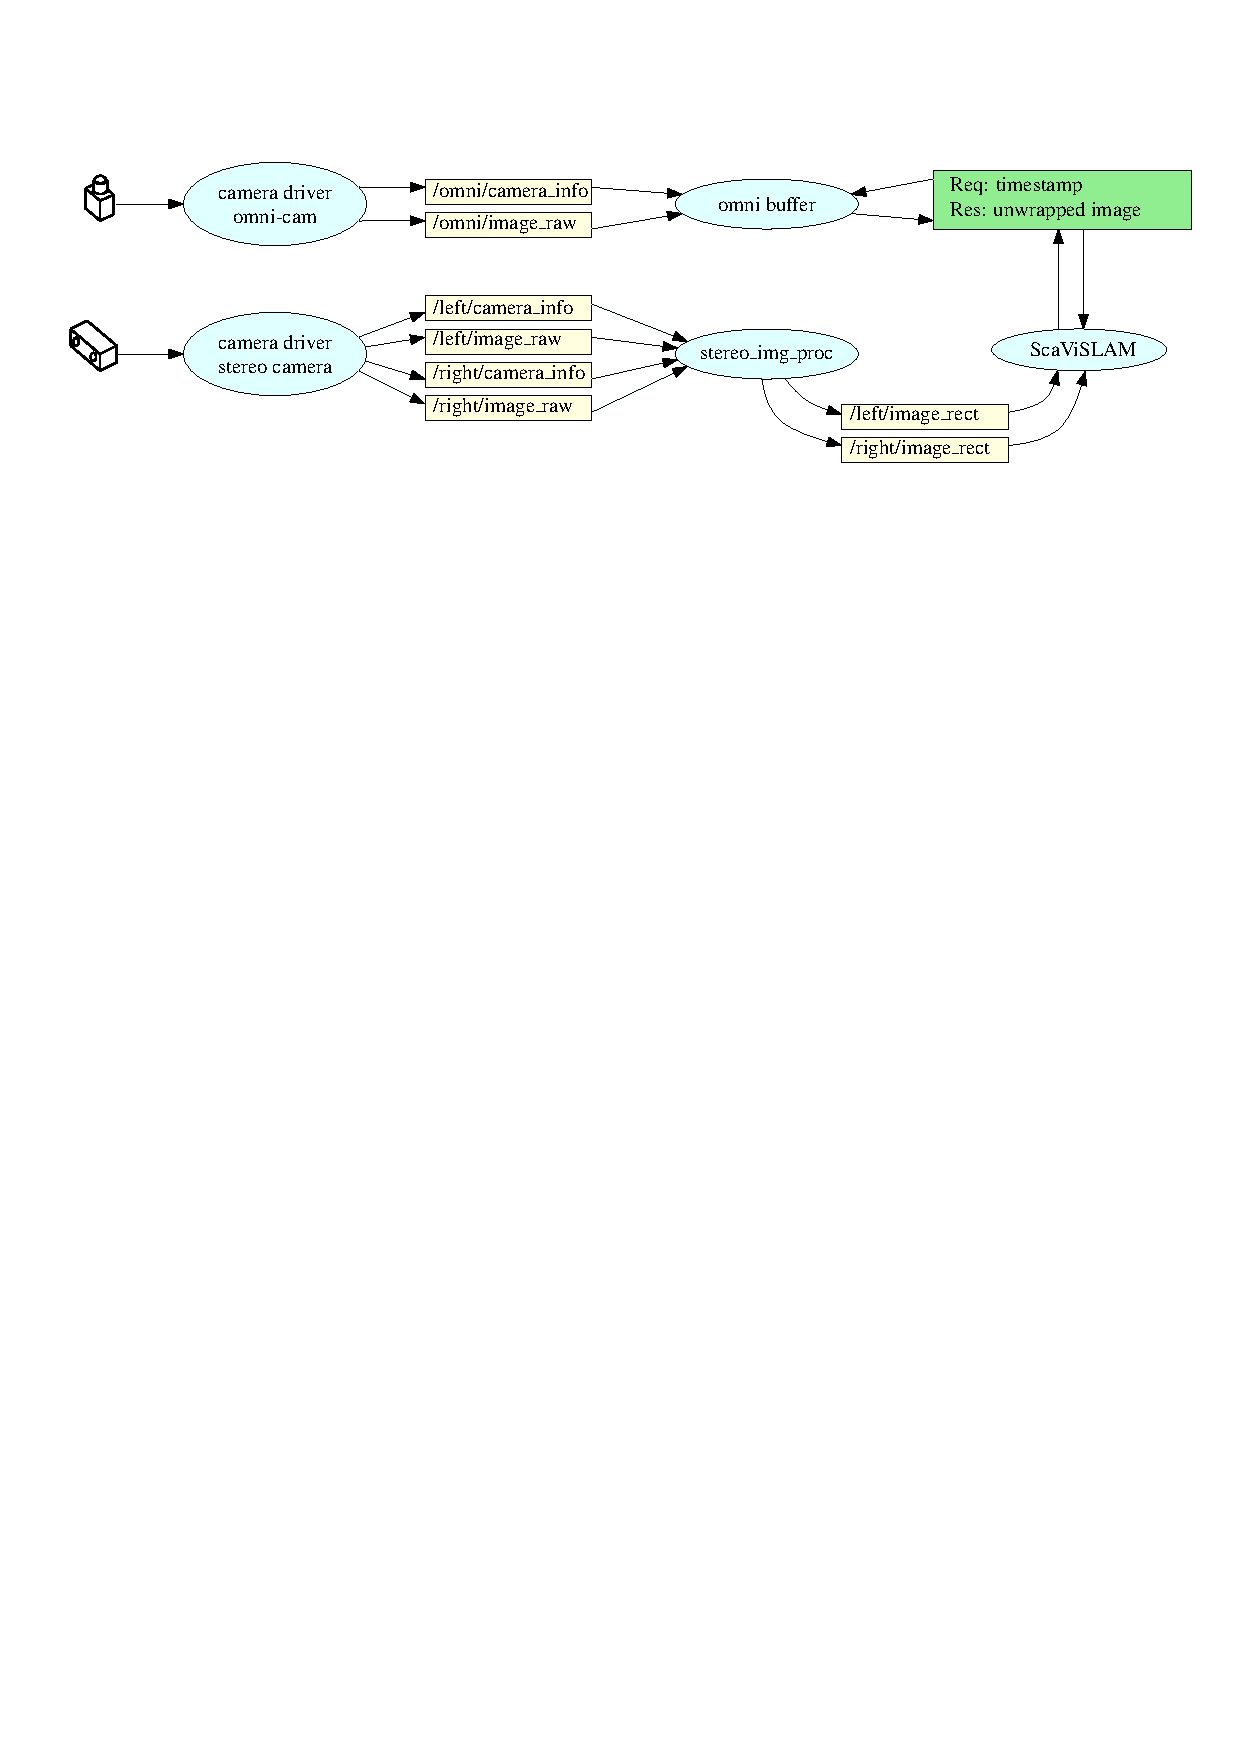
\includegraphics[width=1.1\textwidth]{chapters/images/input_architecture}
  \caption{System diagram for video input to ScaViSLAM system.  Blue are nodes, yellow topics and green services.}
  \label{fig:input_architecture}
\end{figure}

Fig. \ref{fig:input_architecture} outlines the system architecture for the input to ScaViSLAM.  For the stereo camera, a driver node receives data via Ethernet and publishes raw images and camera info.  The stereo image processing node subscribes to these topics, and accepts synchronized frames for processing.  Most importantly, it rectifies the images to non distorted images using the camera intrinsics supplied by camera info. (Sec. \ref{subsec:lense_distortion}) 

The pipeline for the omni camera images is significantly different to the stereo frames.  There are two main reasons for this, one being that there was no hardware synchronization available between omni camera and stereo used in this setup, allowing only approximate synchronization using timestamps.  The second reason was to increase computational efficiency.  There is some computational load associated with unwrapping a donut image to a spherical image.  The omni images are not required for every frame, they are only required for keyframes.  Therefore, only stereo frames which become keyframes require an associated omni camera image.

The omni camera driver receives donut images via firewire and publishes them.  The omni buffer node subscribes to this topic and records every timestamped image to a buffer.  When ScaViSLAM creates a new keyframe, it then queries the omni buffer via a service call, requesting with the timestamp of the stereo frame.  The omni buffer node searches through its buffer for the image closest to this timestamp, unwraps it, and returns it as a response to the service call.

The ROS tool dynamic reconfigure can be used to configure the camera drivers.  This allows adjusting of gain/shutter controls, resolution, image depth etc.

\section{Image based place recognition}

\begin{figure}[H]
  \centering
    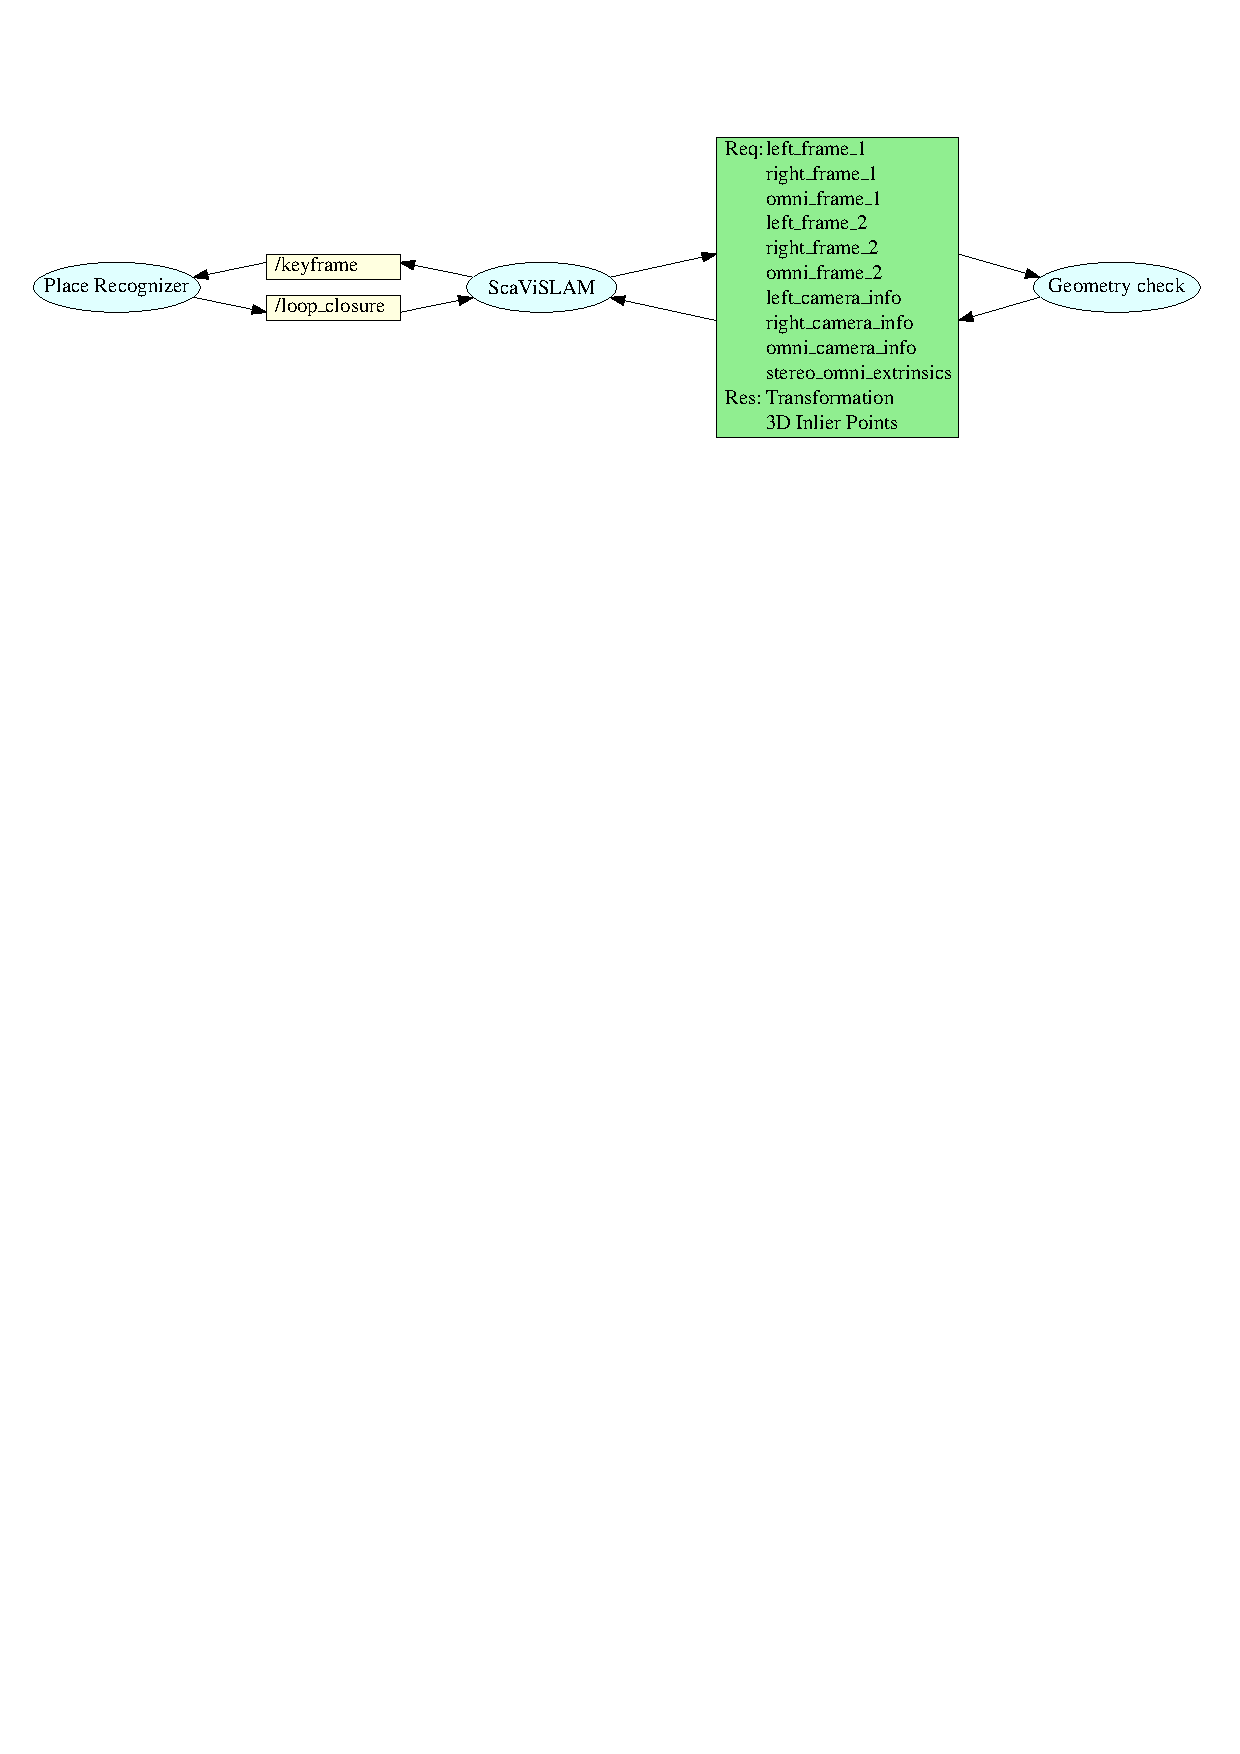
\includegraphics[width=1.1\textwidth]{chapters/images/loop_close_architecture}
  \caption{System diagram for image based loop closure for ScaViSLAM.  Blue are nodes, yellow topics and green services.}
  \label{fig:loop_close_architecture}
\end{figure}

\section{Visualization}


\begin{itemize}
 \item scavislam
 \subitem ros wrapper
 \subitem rviz visualizer
 \subitem dynam reconfig
 \item omni buffer
 \subitem synchronization, unwrapping
 \item place recog
 \subitem modularity
 \item geo check
 \subitem my stuff
\end{itemize}



